\section{Sprint 4 : Maintenance corrective et ordres de travail}

\subsection{Introduction}

Après la maintenance préventive, ce quatrième Sprint est consacré à la maintenance corrective et à la gestion du cycle de vie des ordres de travail.

{\sloppy
La maintenance corrective intervient à la suite d'une panne, d'une anomalie ou d'un dysfonctionnement constaté sur un équipement. Elle nécessite une organisation rigoureuse : le signalement doit être enregistré rapidement, l'intervention doit être affectée à un technicien disponible, les pièces nécessaires doivent être identifiées et l'opération réalisée doit être documentée.
\par}

Ce Sprint vise ainsi à remplacer la gestion manuelle des demandes d'intervention par un processus traçable, depuis le signalement de la panne jusqu'à la clôture de l'ordre de travail. Il s'appuie sur les machines et les modules structurés dans le Sprint 2 ainsi que sur le référentiel préventif développé dans le Sprint 3.

Le chapitre présente les objectifs et le Sprint Backlog, puis la conception du flux correctif. Il décrit ensuite les fonctionnalités réalisées, notamment le signalement, l'affectation, l'exécution et la validation des interventions, avant de présenter les tests de validation.

\subsection{Objectifs du Sprint}

L'objectif principal de ce Sprint est de mettre en place un processus complet de traitement des pannes, depuis leur signalement jusqu'à la clôture de l'ordre de travail correspondant.

Les objectifs spécifiques sont les suivants :

\begin{itemize}
    \item permettre le signalement d'une panne ou d'une anomalie ;
    \item associer le signalement à une machine et, si possible, à un module ;
    \item enregistrer les informations descriptives de la défaillance ;
    \item gérer le référentiel codifié des pannes et les solutions associées ;
    \item créer, affecter et replanifier les ordres de travail ;
    \item permettre au technicien de prendre en charge un ordre de travail ;
    \item gérer les états successifs d'une intervention ;
    \item permettre la demande de pièces et la mise en attente de l'intervention ;
    \item enregistrer les pièces consommées et mettre à jour le stock ;
    \item renseigner le rapport d'intervention ;
    \item clôturer l'intervention et faire valider l'ordre de travail ;
    \item consulter le calendrier, les statistiques et l'historique des interventions.
\end{itemize}

\subsection{Sprint Backlog}

Le tableau~\ref{tab:sprint4-backlog} recense les tâches planifiées pour ce Sprint.

{\footnotesize
\setlength{\tabcolsep}{4pt}
\begin{longtable}{|p{0.9cm}|p{10.9cm}|p{1.4cm}|p{1.4cm}|}
\caption{Sprint Backlog du Sprint 4}
\label{tab:sprint4-backlog}\\
\hline
\textbf{ID} & \textbf{Tâche} & \textbf{Priorité} & \textbf{Statut} \\
\hline
\endfirsthead

\hline
\textbf{ID} & \textbf{Tâche} & \textbf{Priorité} & \textbf{Statut} \\
\hline
\endhead

S4-01 &
Développer le signalement d'une panne et la création de l'ordre de travail associé. &
Haute & Réalisé \\
\hline

S4-02 &
Gérer le référentiel des pannes et les solutions correctives. &
Moyenne & Réalisé \\
\hline

S4-03 &
Développer la création, la modification et l'affectation des ordres de travail. &
Haute & Réalisé \\
\hline

S4-04 &
Mettre en place le calendrier et la replanification des ordres de travail. &
Moyenne & Réalisé \\
\hline

S4-05 &
Développer la prise en charge et le démarrage d'une intervention. &
Haute & Réalisé \\
\hline

S4-06 &
Gérer la mise en attente pour indisponibilité de pièces. &
Haute & Réalisé \\
\hline

S4-07 &
Développer les demandes de pièces et leur décision. &
Haute & Réalisé \\
\hline

S4-08 &
Enregistrer les pièces consommées et décrémenter le stock. &
Haute & Réalisé \\
\hline

S4-09 &
Développer le rapport du technicien et la clôture de l'intervention. &
Haute & Réalisé \\
\hline

S4-10 &
Mettre en place la validation de l'ordre de travail et les statistiques associées. &
Haute & Réalisé \\
\hline

S4-11 &
Intégrer l'assistant correctif et les recommandations d'aide au diagnostic. &
Moyenne & Réalisé \\
\hline

S4-12 &
Vérifier le flux correctif par des tests d'API et des tests automatisés. &
Haute & Réalisé \\
\hline

\end{longtable}}

User Stories associées :

\begin{itemize}
    \item \textbf{US12 :} en tant qu'opérateur, je souhaite signaler une panne afin de déclencher une intervention corrective ;
    \item \textbf{US13 :} en tant qu'administrateur, je souhaite créer et affecter un ordre de travail afin d'organiser les interventions ;
    \item \textbf{US14 :} en tant que technicien, je souhaite prendre en charge et exécuter un ordre de travail afin de rétablir le fonctionnement de l'équipement ;
    \item \textbf{US15 :} en tant que technicien, je souhaite demander des pièces et déclarer leur consommation afin d'assurer le suivi du stock ;
    \item \textbf{US16 :} en tant que technicien, je souhaite renseigner un rapport d'intervention afin de conserver la trace des opérations réalisées ;
    \item \textbf{US17 :} en tant qu'administrateur, je souhaite valider et clôturer un ordre de travail afin de contrôler la qualité du traitement.
\end{itemize}

\subsection{Conception du Sprint}

\subsubsection{Diagramme des cas d'utilisation}

Le diagramme de la figure~\ref{fig:usecase-corrective} présente les cas d'utilisation du flux correctif. L'opérateur signale une panne, ce qui déclenche la création d'un ordre de travail. L'administrateur gère le référentiel des pannes et des solutions, crée et affecte les ordres de travail, valide leur clôture et consulte le calendrier et les statistiques. Le technicien prend en charge un ordre de travail, exécute l'intervention, demande les pièces nécessaires, déclare celles qui sont consommées et renseigne le rapport d'intervention. Un acteur optionnel, l'assistant IA, accompagne le diagnostic technique sans se substituer à la décision de l'administrateur ou du technicien.

\begin{figure}[H]
    \centering
    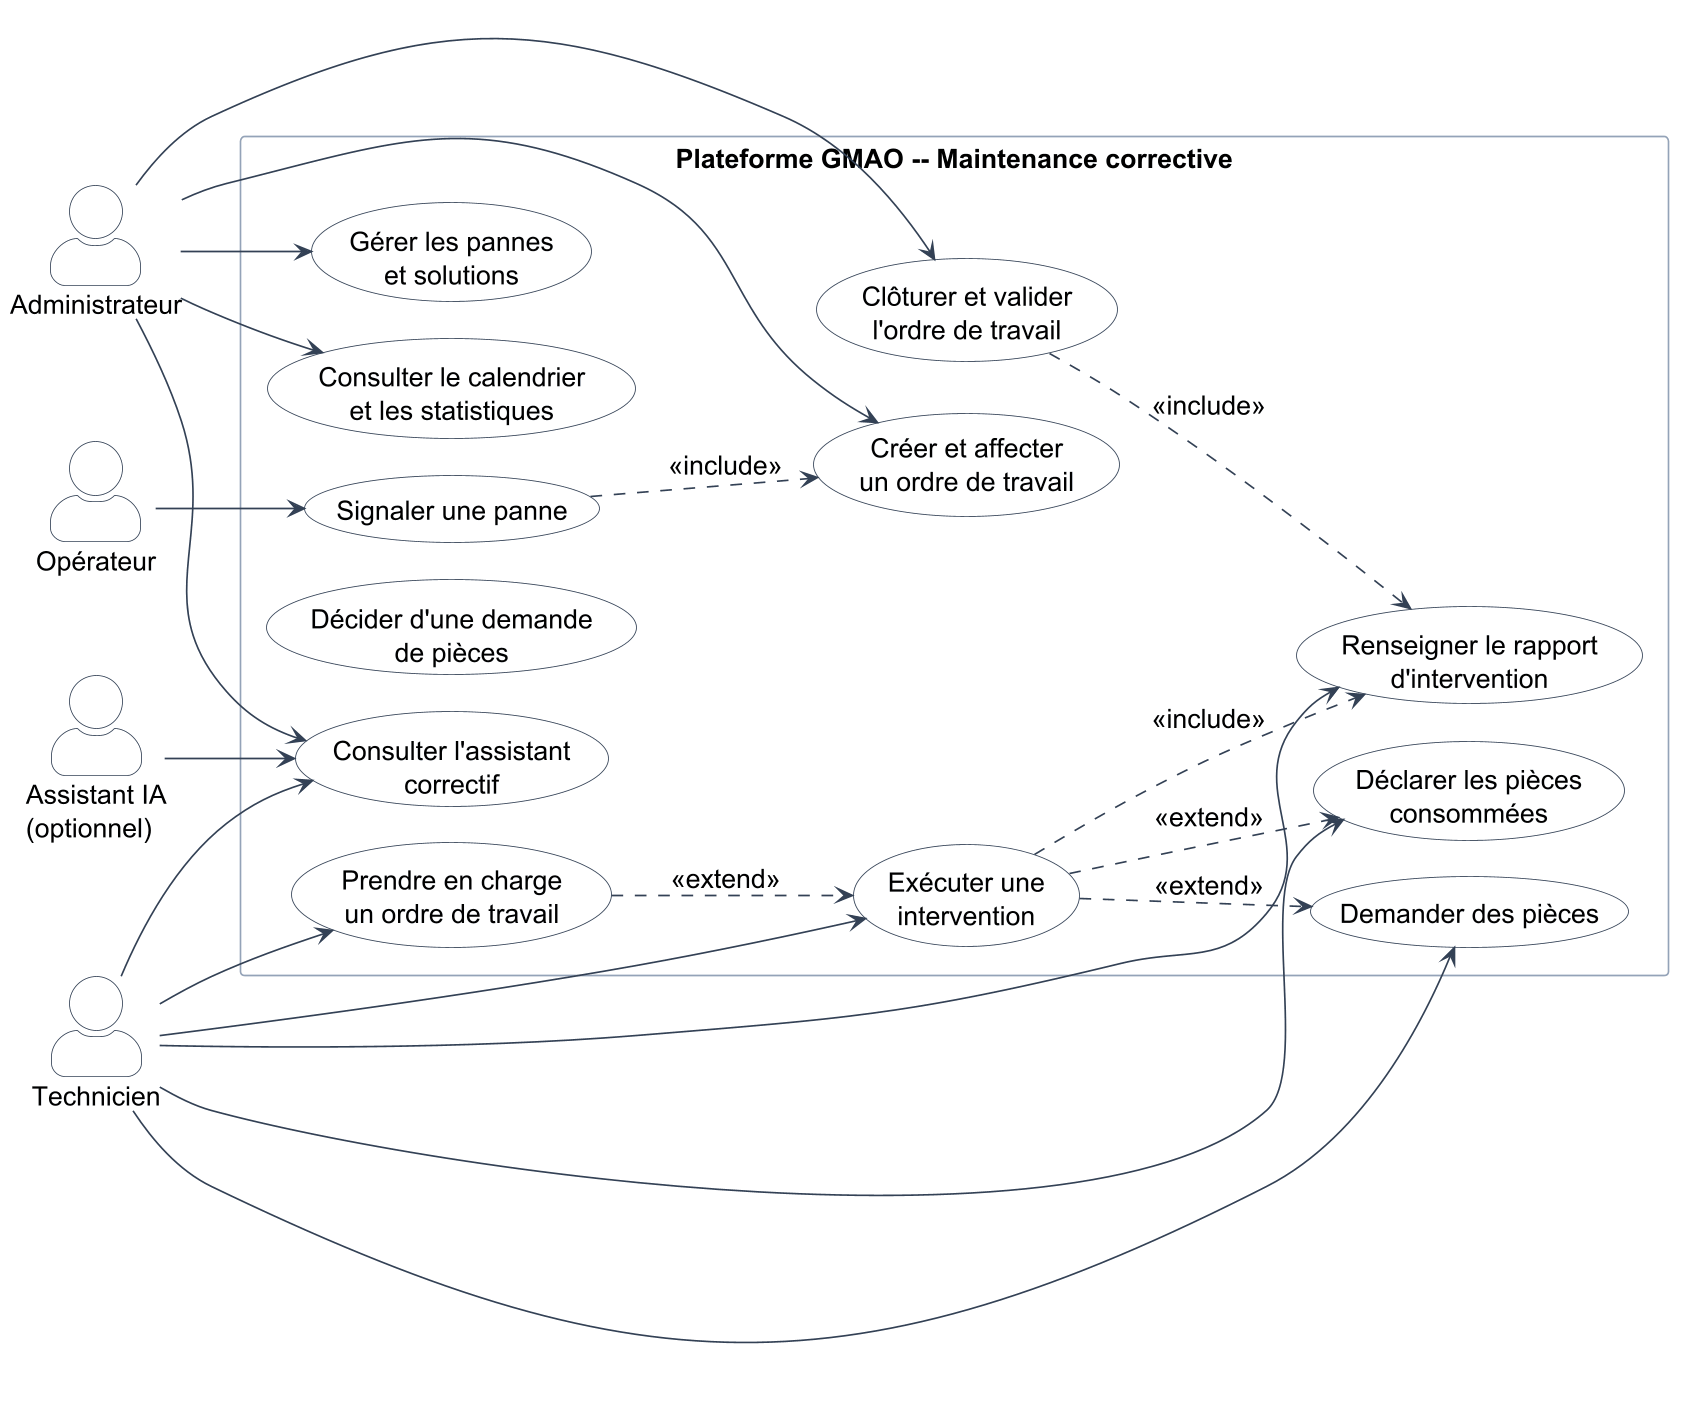
\includegraphics[width=0.92\textwidth,height=0.78\textheight,keepaspectratio]{figures/usecase-corrective.png}
    \caption{Diagramme des cas d'utilisation du Sprint 4}
    \label{fig:usecase-corrective}
\end{figure}

\subsubsection{Diagramme d'activités du flux correctif}

La figure~\ref{fig:activity-corrective} présente le déroulement d'une intervention corrective, depuis le signalement jusqu'à la validation de l'ordre de travail. Le flux prévoit une attente lorsque les pièces nécessaires ne sont pas disponibles.

\begin{figure}[H]
    \centering
    \IfFileExists{figures/activity-corrective.png}{%
        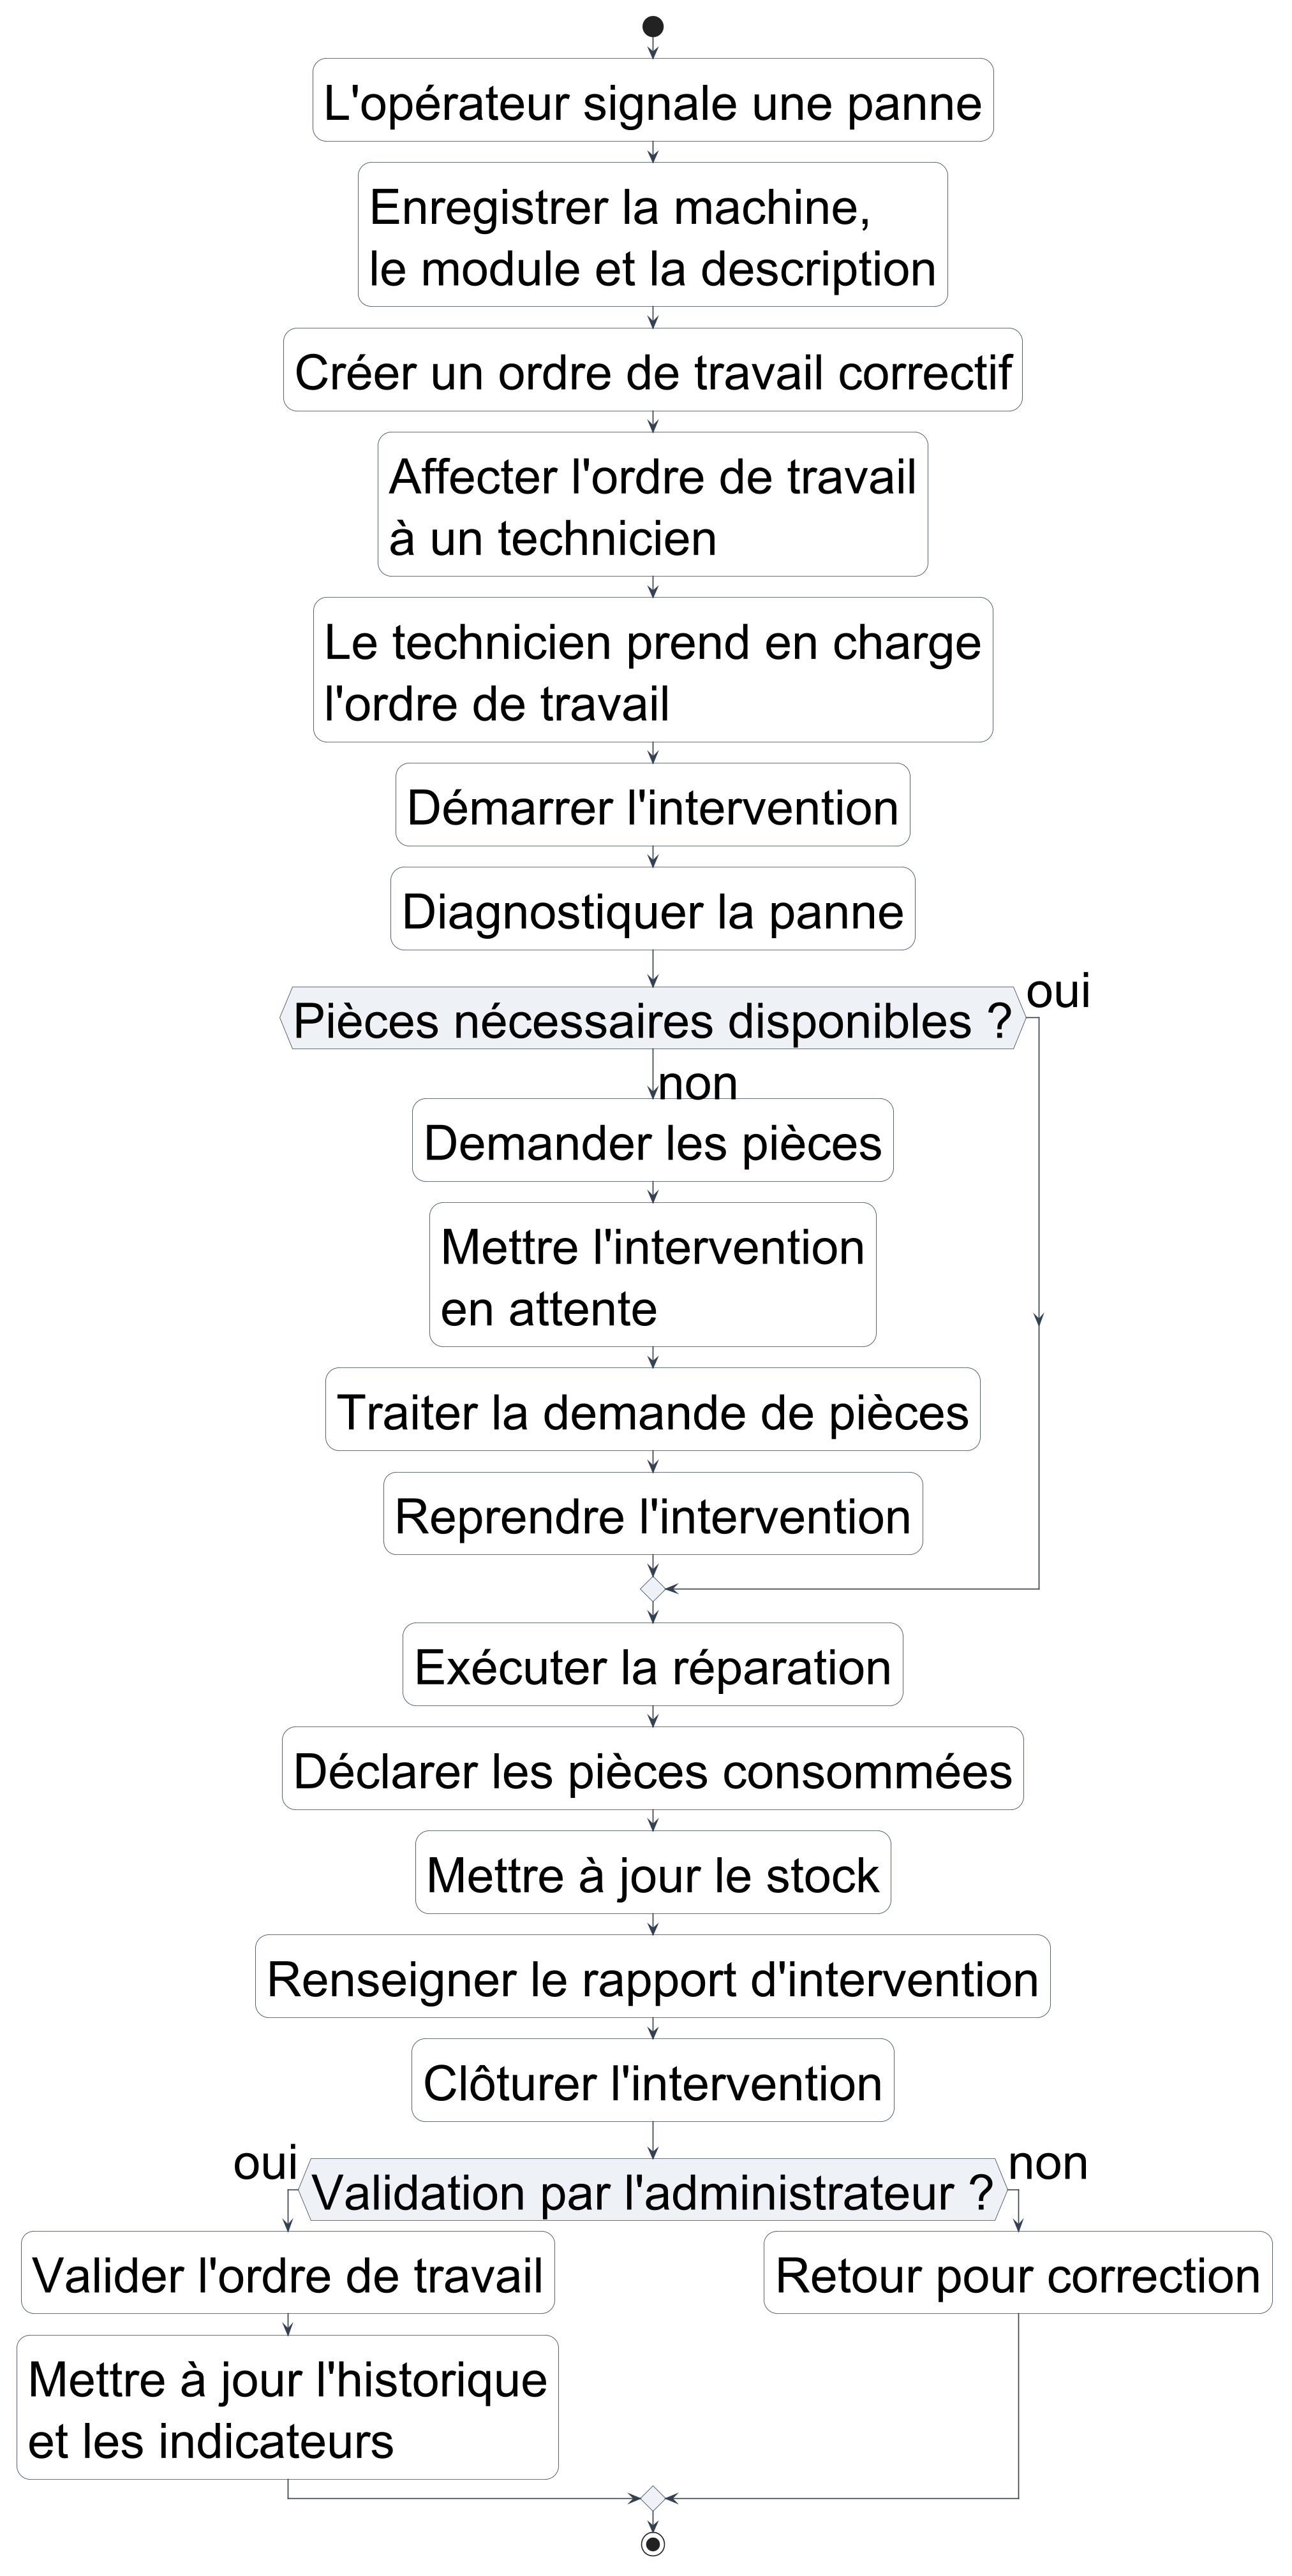
\includegraphics[width=0.85\textwidth,height=0.86\textheight,keepaspectratio]{figures/activity-corrective.png}%
    }{%
        \fbox{\parbox[c][7cm][c]{0.92\textwidth}{\centering\itshape Diagramme à insérer\\[2mm]\texttt{figures/activity-corrective.png}}}%
    }
    \caption{Diagramme d'activités du flux de maintenance corrective}
    \label{fig:activity-corrective}
\end{figure}

\subsubsection{Diagramme d'états d'un ordre de travail}

L'ordre de travail évolue selon une succession d'états contrôlés. La figure~\ref{fig:state-work-order} présente son cycle de vie.

\begin{figure}[H]
    \centering
    \IfFileExists{figures/state-work-order.png}{%
        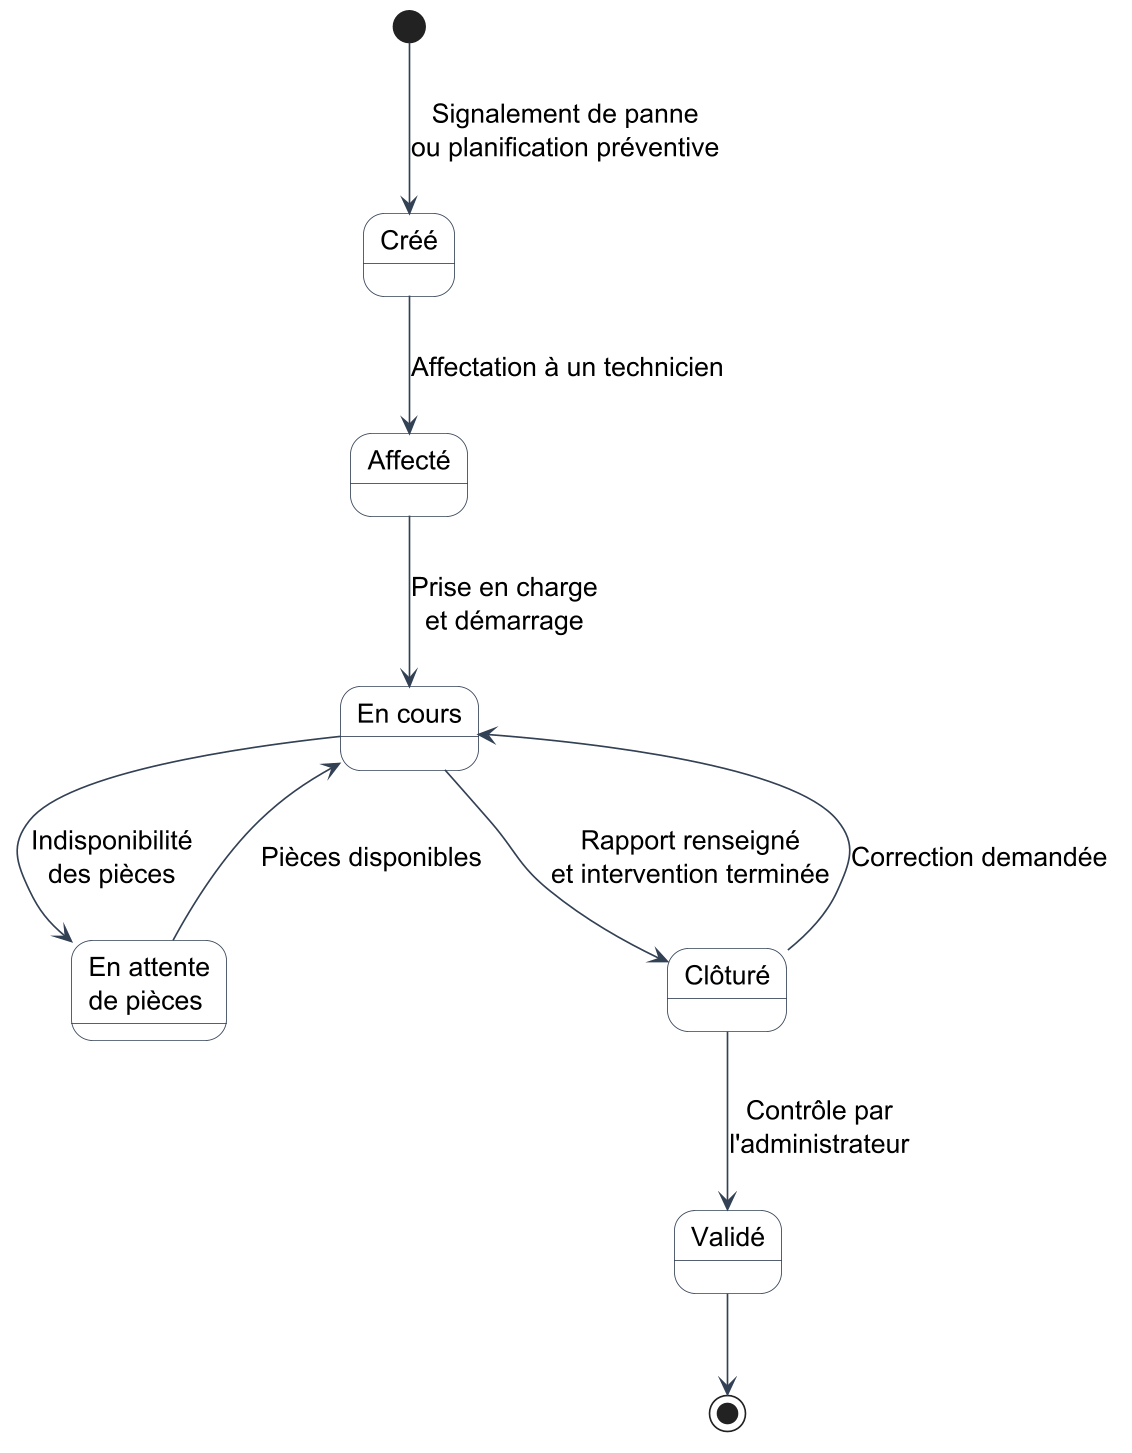
\includegraphics[width=0.85\textwidth,height=0.82\textheight,keepaspectratio]{figures/state-work-order.png}%
    }{%
        \fbox{\parbox[c][7cm][c]{0.92\textwidth}{\centering\itshape Diagramme à insérer\\[2mm]\texttt{figures/state-work-order.png}}}%
    }
    \caption{Diagramme d'états d'un ordre de travail}
    \label{fig:state-work-order}
\end{figure}

Un ordre de travail peut être créé à la suite d'un signalement de panne ou d'une planification préventive. Il est ensuite affecté à un technicien, qui le prend en charge et démarre l'intervention. Si les pièces nécessaires sont indisponibles, l'ordre passe en attente puis reprend l'exécution dès leur réception.

La clôture n'est prononcée qu'après le renseignement du rapport d'intervention. L'administrateur contrôle ensuite le travail réalisé : il valide l'ordre de travail, ce qui met à jour l'historique et les indicateurs, ou demande une correction qui le replace en cours d'exécution.

\subsubsection{Diagramme de séquence de l'intervention corrective}

La figure~\ref{fig:sequence-corrective} présente les échanges entre le technicien, l'interface, l'API et le service de stock lors du traitement d'une intervention.

\begin{figure}[H]
    \centering
    \IfFileExists{figures/sequence-corrective.png}{%
        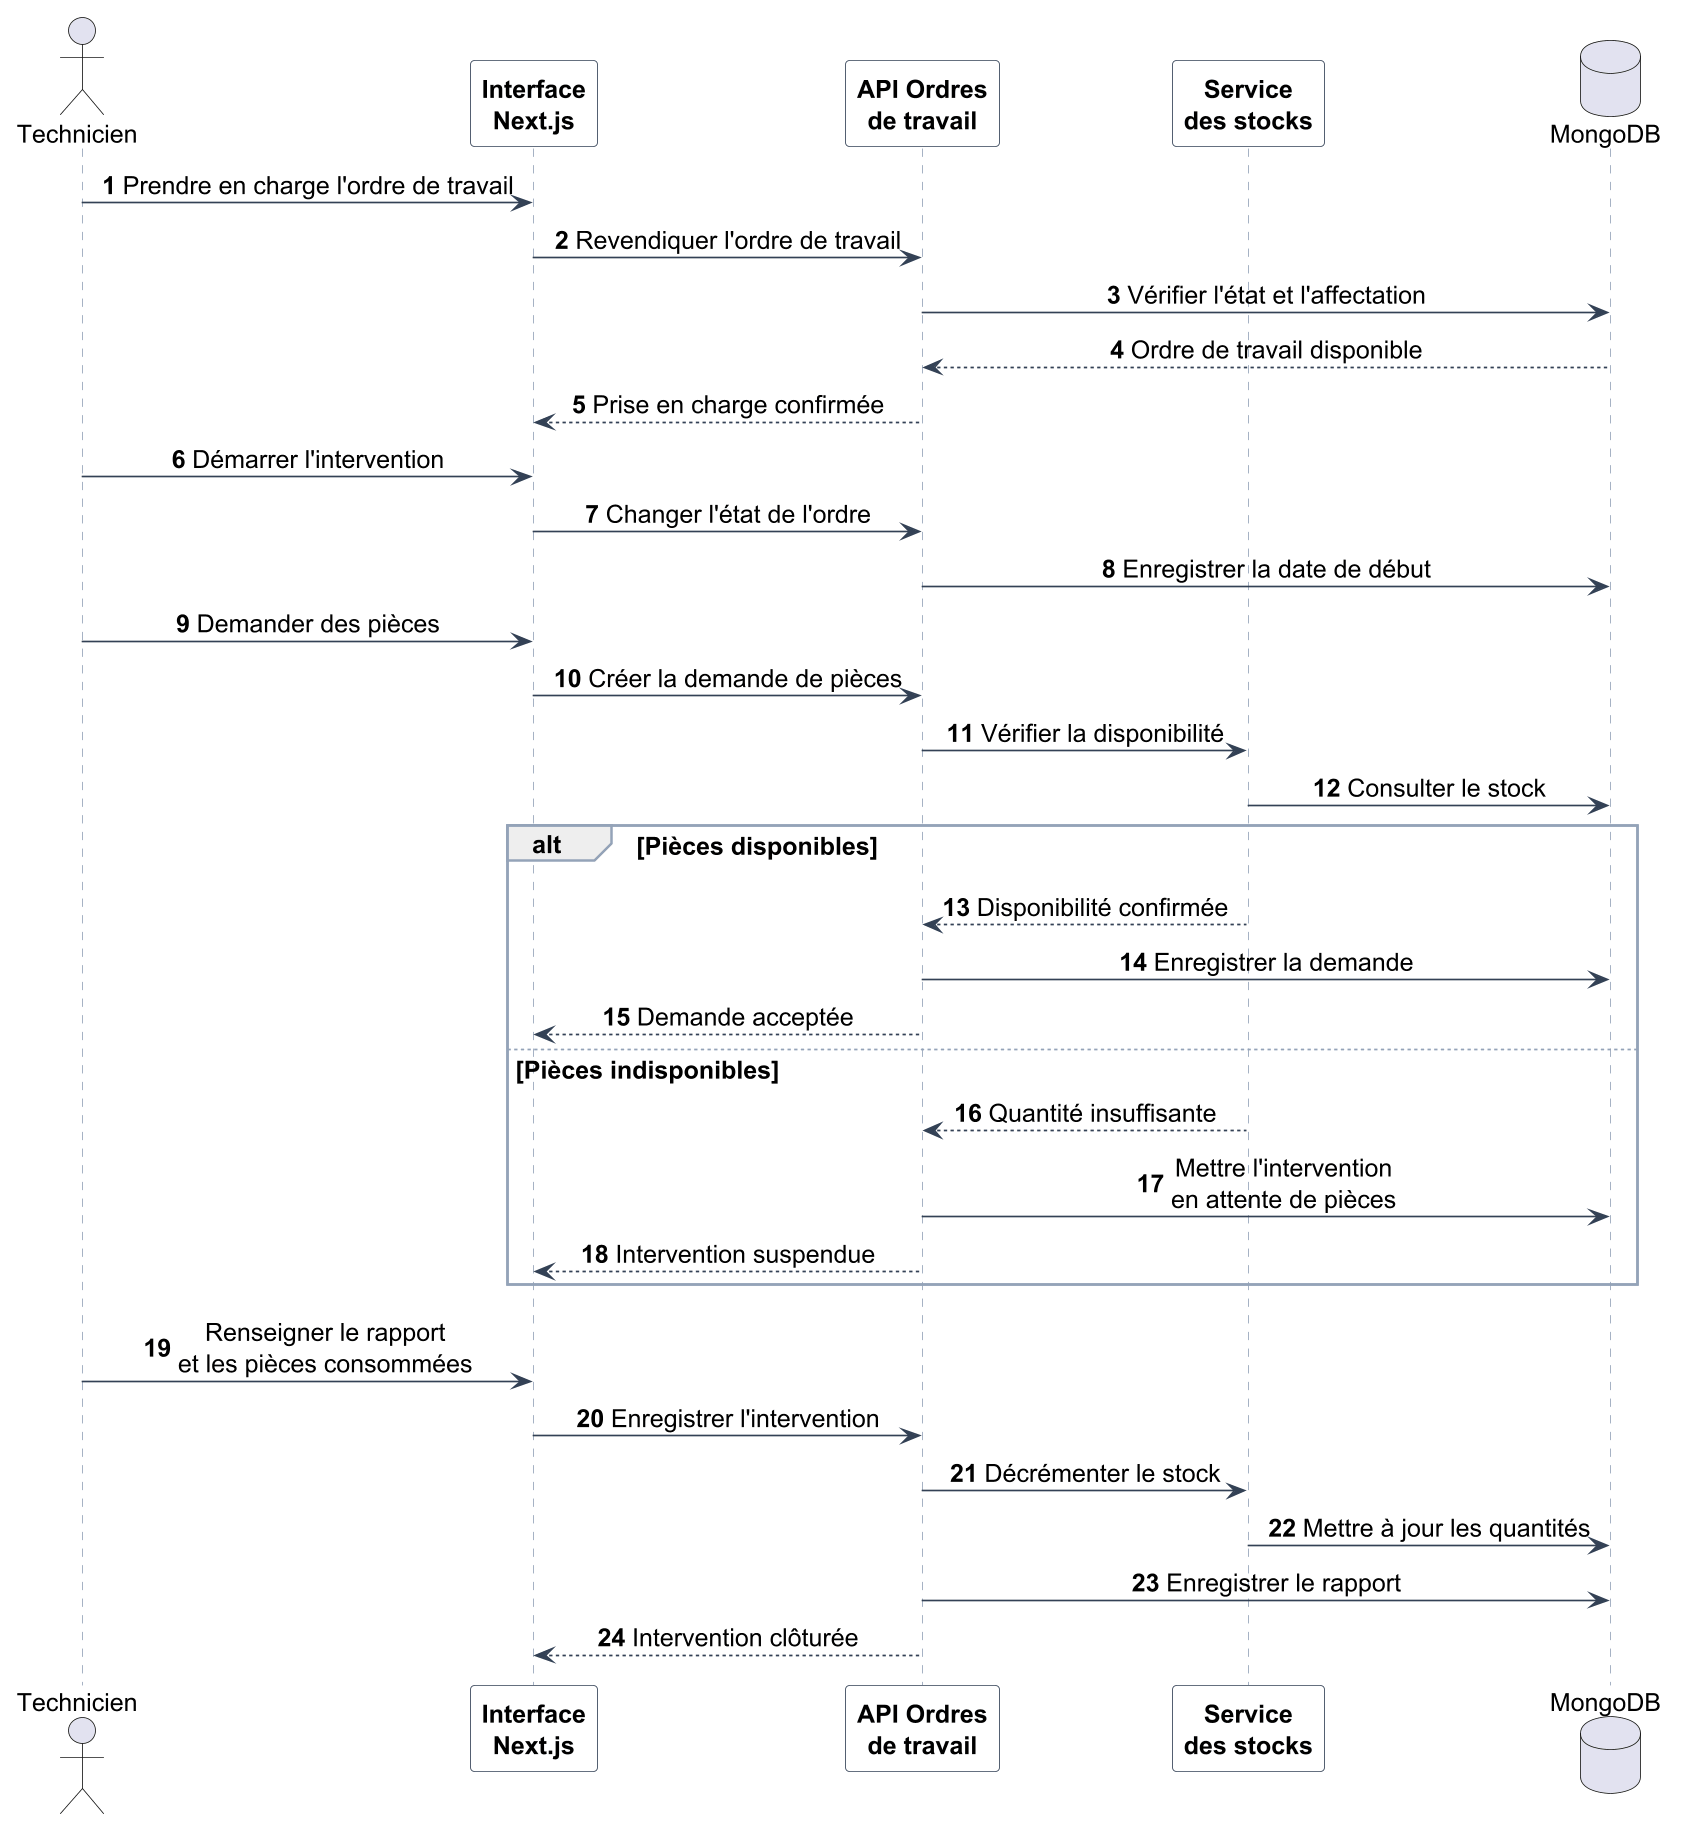
\includegraphics[width=\textwidth,height=0.78\textheight,keepaspectratio]{figures/sequence-corrective.png}%
    }{%
        \fbox{\parbox[c][7cm][c]{0.92\textwidth}{\centering\itshape Diagramme à insérer\\[2mm]\texttt{figures/sequence-corrective.png}}}%
    }
    \caption{Diagramme de séquence du traitement d'une intervention corrective}
    \label{fig:sequence-corrective}
\end{figure}

La prise en charge vérifie d'abord que l'ordre de travail est bien affecté au technicien et qu'il n'a pas déjà été revendiqué. Le démarrage enregistre la date de début de l'intervention.

Lors d'une demande de pièces, la disponibilité est contrôlée auprès du service des stocks. Si la quantité est suffisante, la demande est enregistrée et le technicien est notifié ; sinon, l'intervention passe en attente de pièces jusqu'à leur réapprovisionnement. À la clôture, les pièces consommées sont décrémentées du stock et le rapport d'intervention est conservé avec l'ordre de travail.

\subsubsection{Modèle de données du flux correctif}

Le tableau~\ref{tab:modele-corrective} présente les principales entités du flux correctif et leur rôle.

\begin{table}[H]
\centering
\caption{Entités du flux de maintenance corrective}
\label{tab:modele-corrective}
\small
\begin{tabularx}{\textwidth}{|p{3.2cm}|X|}
\hline
\textbf{Entité} & \textbf{Rôle dans le domaine} \\
\hline
\texttt{Fault} & Référentiel codifié des pannes et des causes recensées \\
\hline
\texttt{FaultSolution} & Solution ou procédure corrective associée à une panne \\
\hline
\texttt{WorkOrder} & Ordre de travail reliant une machine, un module, un technicien et une intervention \\
\hline
\texttt{InterventionReport} & Rapport détaillant les opérations réalisées et la durée de l'intervention \\
\hline
\texttt{PartRequest} & Demande de pièces associée à un ordre de travail \\
\hline
\texttt{Catalogue} & Référentiel des pièces de rechange disponibles \\
\hline
\texttt{Stock} & Quantités disponibles et réservées pour chaque pièce \\
\hline
\texttt{Notification} & Information transmise aux acteurs concernés \\
\hline
\end{tabularx}
\end{table}

Un ordre de travail est rattaché à une machine et, lorsque l'information existe, à un module. Il peut être lié à un plan préventif ou à un signalement correctif. Le technicien affecté et le rapport d'intervention permettent de suivre l'exécution.

Les demandes de pièces relient l'ordre de travail au catalogue. La consommation effective entraîne une mise à jour du stock et conserve la trace du mouvement.

\subsection{Réalisation}

\subsubsection{Signalement d'une panne}

Depuis son espace de travail, l'opérateur sélectionne la machine concernée puis décrit l'anomalie constatée, son contexte et, lorsque cela est possible, le module en cause.

Le signalement peut être rapproché du référentiel des pannes afin d'identifier un code de défaillance. Cette codification facilite le regroupement des incidents, l'analyse des causes fréquentes et le calcul des indicateurs de maintenance.

Une fois le signalement enregistré, un ordre de travail correctif est créé. Selon l'organisation retenue, il peut être affecté directement à un technicien ou rester disponible pour une prise en charge.

Le formulaire de signalement guide l'opérateur dans le choix de la machine et du module, la description de l'anomalie et la saisie du code de panne.

\begin{figure}[H]
    \centering
    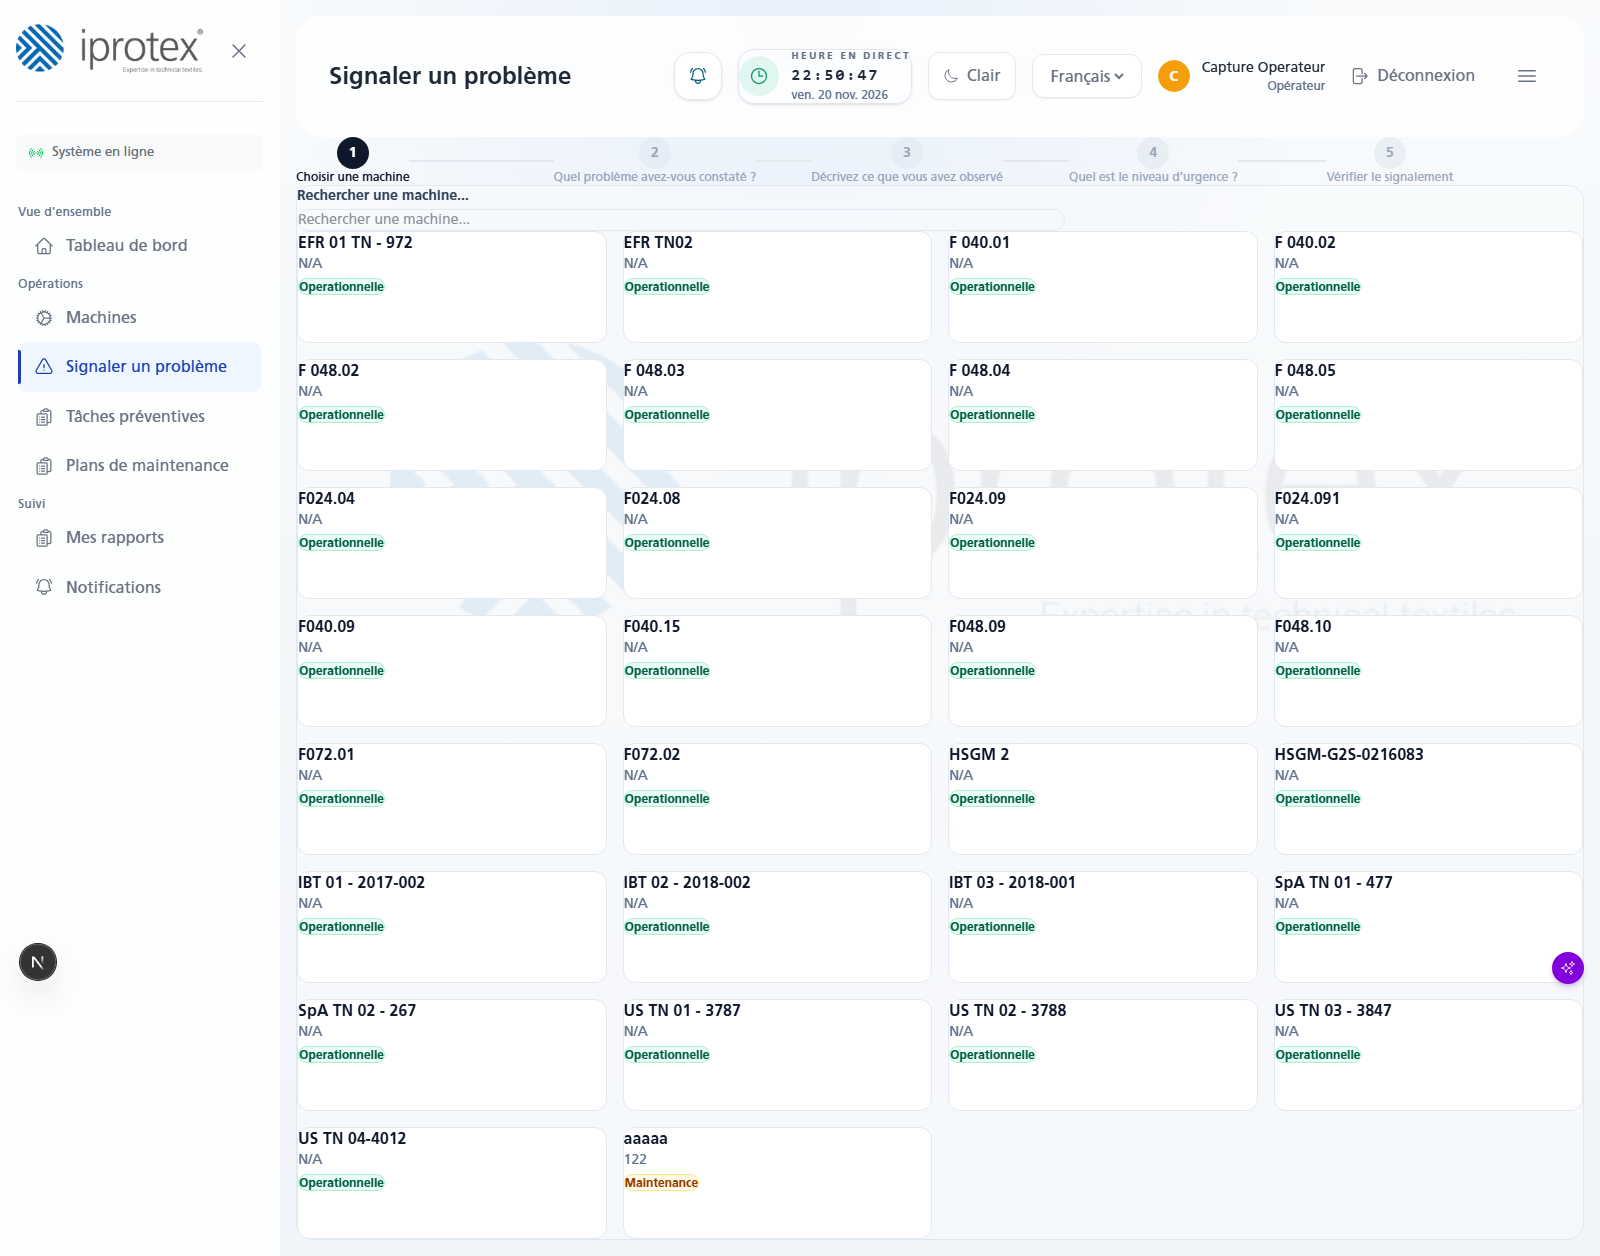
\includegraphics[width=0.80\textwidth,height=0.76\textheight,keepaspectratio]{figures/captures/sprint4-panne.png}
    \caption{Formulaire de signalement d'une panne}
    \label{fig:sprint4-panne}
\end{figure}

\subsubsection{Gestion des ordres de travail}

L'administrateur peut créer un ordre de travail, le modifier, le supprimer ou le replanifier. Chaque ordre précise la machine concernée, le module éventuel, la priorité, la date prévue, le technicien affecté et l'origine de l'intervention.

Le calendrier des ordres de travail offre une vue sur les interventions planifiées. Il facilite la répartition de la charge et permet d'ajuster les dates en cas de contrainte opérationnelle.

Les statistiques regroupent notamment le nombre d'ordres créés, d'interventions en cours, d'ordres en attente de pièces et d'interventions clôturées. Ces informations alimentent les tableaux de bord présentés dans le Sprint suivant.

    La liste des ordres de travail affiche la priorité, le technicien affecté, l'état et l'échéance de chaque intervention.

\begin{figure}[H]
    \centering
    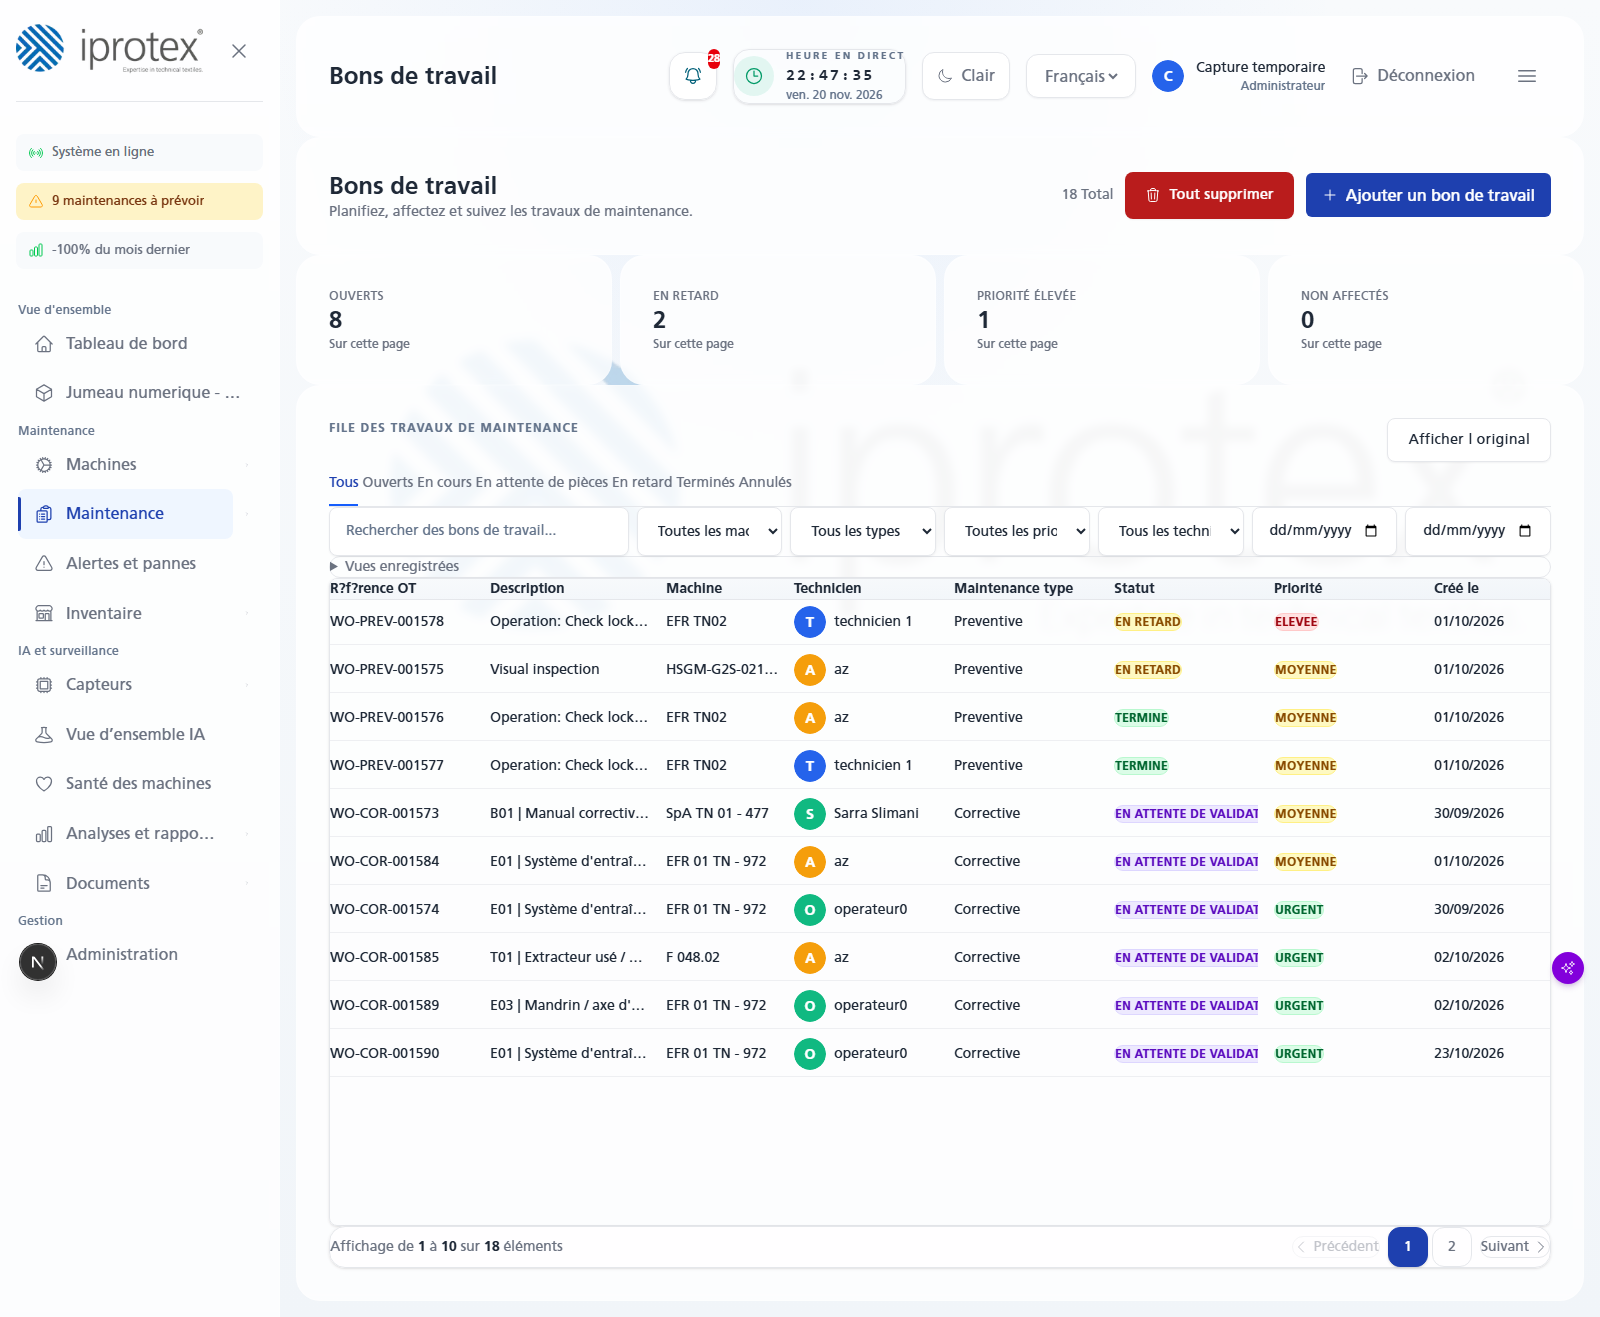
\includegraphics[width=0.88\textwidth,height=0.78\textheight,keepaspectratio]{figures/captures/sprint4-work-orders.png}
    \caption{Suivi des ordres de travail}
    \label{fig:sprint4-work-orders}
\end{figure}

\subsubsection{Prise en charge et exécution}

Le technicien consulte les ordres de travail qui lui sont affectés ou qui sont disponibles. Il prend en charge l'intervention, puis la démarre lorsque les conditions le permettent.

Au cours de l'intervention, il peut :

\begin{itemize}
    \item consulter l'historique et les documents techniques de la machine ;
    \item diagnostiquer la panne et consulter les solutions associées ;
    \item demander les pièces nécessaires ;
    \item mettre l'intervention en attente si une pièce n'est pas disponible ;
    \item reprendre le travail une fois les pièces obtenues ;
    \item indiquer les quantités de pièces utilisées ;
    \item renseigner les opérations réalisées et les observations ;
    \item clôturer l'intervention.
\end{itemize}

La mise en attente conserve la cause du blocage. Elle permet de distinguer une intervention retardée par une rupture de stock d'une intervention simplement non démarrée.

Lorsqu'une pièce n'est pas disponible, l'intervention est suspendue : l'écran conserve la pièce demandée, sa quantité, son statut et l'action de reprise.

\begin{figure}[H]
    \centering
    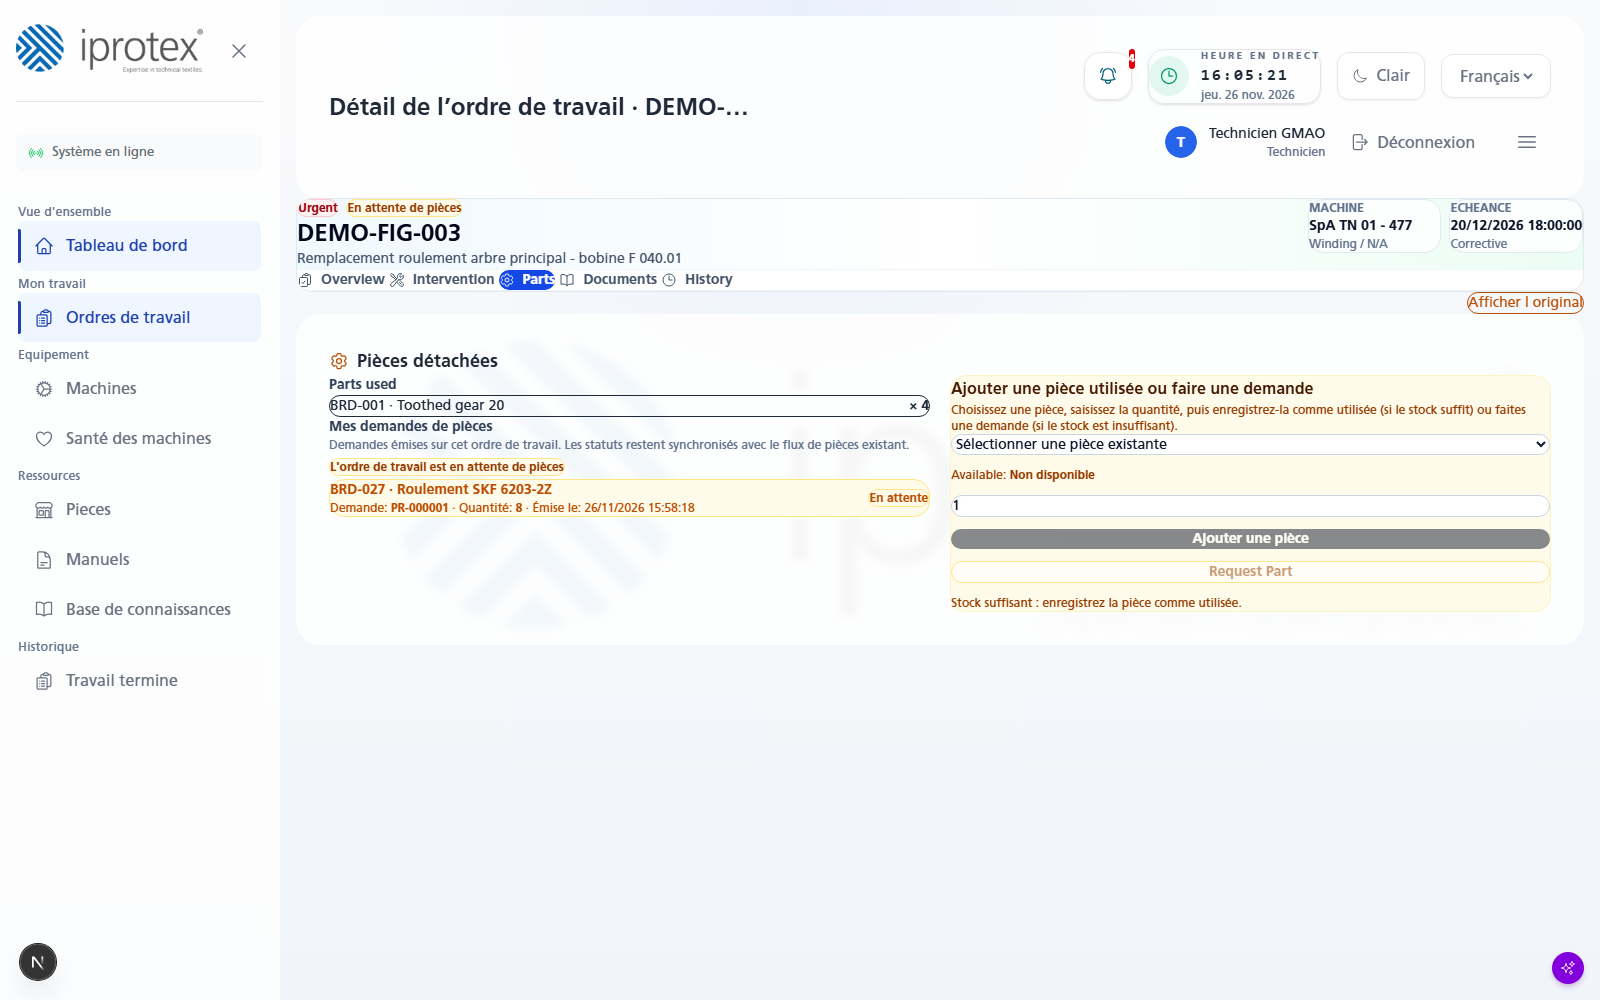
\includegraphics[width=0.92\textwidth,height=0.72\textheight,keepaspectratio]{figures/captures/sprint4-waiting-parts.png}
    \caption{Intervention suspendue pour indisponibilité de pièces}
    \label{fig:sprint4-waiting-parts}
\end{figure}

\subsubsection{Demande et consommation des pièces}

La demande de pièces précise la référence, la quantité souhaitée et l'ordre de travail concerné. Elle est soumise à une décision qui peut l'accepter, la réserver ou la refuser selon la disponibilité et les règles de gestion définies.

Lorsque la demande est acceptée et que l'intervention est réalisée, la consommation effective est enregistrée. Cette opération décrémente le stock disponible, conserve le mouvement et rattache la pièce à l'ordre de travail.

Ce mécanisme assure la traçabilité des pièces utilisées et permet de calculer ultérieurement le coût des interventions. La gestion détaillée du catalogue et des mouvements de stock est approfondie dans le Sprint 5.

\subsubsection{Rapport d'intervention et clôture}

Le rapport d'intervention regroupe les informations relatives à l'opération réalisée : dates de début et de fin, diagnostic, actions effectuées, pièces utilisées et observations.

Le technicien renseigne ce rapport avant de clôturer l'intervention. L'ordre de travail passe alors dans un état permettant le contrôle par l'administrateur.

La validation de l'ordre de travail confirme que l'intervention a été correctement documentée. Elle met à jour l'historique de la machine et alimente les indicateurs de maintenance, notamment le temps moyen de réparation.

    Le rapport d'intervention documente le diagnostic, les actions réalisées, les pièces utilisées et les durées de l'intervention.

\begin{figure}[H]
    \centering
    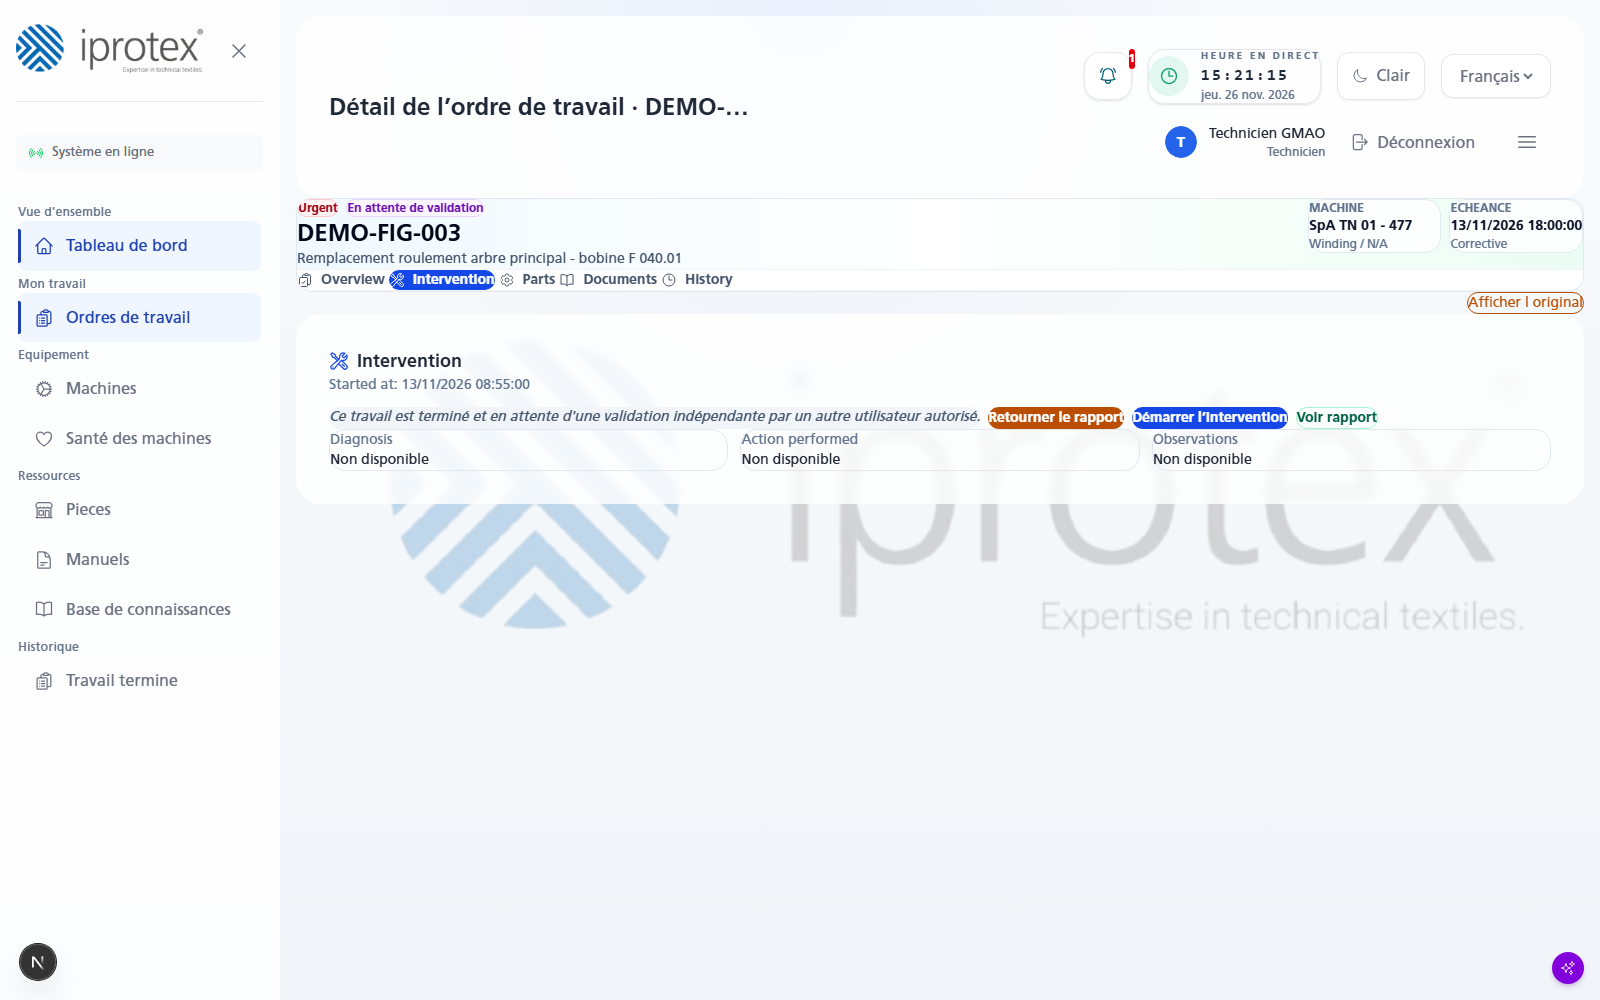
\includegraphics[width=0.92\textwidth,height=0.72\textheight,keepaspectratio]{figures/captures/sprint4-intervention-report.png}
    \caption{Rapport d'intervention corrective}
    \label{fig:sprint4-intervention-report}
\end{figure}

\subsubsection{Assistant correctif}

La plateforme propose un assistant d'aide au diagnostic destiné aux interventions correctives. Il s'appuie sur l'historique des interventions, le référentiel des pannes et les solutions déjà enregistrées.

L'assistant peut suggérer une piste de diagnostic ou une procédure à partir du contexte de la machine et de la panne signalée. Il conserve également l'historique des interactions afin de permettre la consultation des recommandations précédentes.

Cette fonctionnalité constitue une aide à la décision. Les recommandations produites ne remplacent pas le diagnostic du technicien ni la validation de l'administrateur.

L'activation de l'assistant dépend de la configuration du service correspondant. Lorsqu'il est désactivé, le reste du flux correctif demeure pleinement opérationnel.

\subsection{Tests et validation}

Le tableau~\ref{tab:tests-sprint4} présente une synthèse des scénarios vérifiés pour ce Sprint.

{\footnotesize
\setlength{\tabcolsep}{4pt}
\begin{longtable}{|p{0.9cm}|>{\raggedright\arraybackslash}p{7cm}|>{\raggedright\arraybackslash}p{4.7cm}|}
\caption{Scénarios de test du Sprint 4}
\label{tab:tests-sprint4}\\
\hline
\textbf{ID} & \textbf{Scénario} & \textbf{Résultat attendu} \\
\hline
\endfirsthead

\hline
\textbf{ID} & \textbf{Scénario} & \textbf{Résultat attendu} \\
\hline
\endhead

T4-01 &
Signalement d'une panne par un opérateur &
Ordre de travail correctif créé \\
\hline

T4-02 &
Signalement sans machine sélectionnée &
Enregistrement refusé \\
\hline

T4-03 &
Création d'un ordre de travail et affectation à un technicien &
Ordre visible dans l'espace du technicien \\
\hline

T4-04 &
Prise en charge d'un ordre déjà affecté &
Action refusée \\
\hline

T4-05 &
Démarrage d'une intervention &
État et date de début enregistrés \\
\hline

T4-06 &
Demande de pièces disponibles &
Demande acceptée et réservation enregistrée \\
\hline

T4-07 &
Demande de pièces indisponibles &
Intervention mise en attente \\
\hline

T4-08 &
Reprise après disponibilité des pièces &
Intervention de nouveau en cours \\
\hline

T4-09 &
Déclaration des pièces consommées &
Stock décrémenté et mouvement conservé \\
\hline

T4-10 &
Renseignement du rapport et clôture &
Intervention clôturée en attente de validation \\
\hline

T4-11 &
Validation par l'administrateur &
Ordre validé et historique mis à jour \\
\hline

T4-12 &
Replanification d'un ordre de travail &
Nouvelle date visible dans le calendrier \\
\hline

T4-13 &
Consultation de l'assistant correctif désactivé &
Message explicite sans blocage du flux \\
\hline

\end{longtable}}

Les tests ont confirmé la cohérence du flux correctif, notamment le passage par l'attente de pièces, la mise à jour du stock après consommation et l'exigence de validation avant la clôture définitive.

\subsection{Revue du Sprint et conclusion}

Lors de la revue, le signalement d'une panne, la création et l'affectation d'un ordre de travail, l'exécution par le technicien, la gestion des pièces et la validation ont été présentés.

Les principaux résultats du Sprint sont les suivants :

\begin{itemize}
    \item mise en place du signalement des pannes par les opérateurs ;
    \item création, affectation, replanification et suivi des ordres de travail ;
    \item gestion des états successifs d'une intervention ;
    \item prise en charge et exécution des interventions par les techniciens ;
    \item gestion des demandes de pièces et mise en attente pour indisponibilité ;
    \item enregistrement des pièces consommées et mise à jour du stock ;
    \item production des rapports d'intervention ;
    \item validation des ordres de travail et alimentation de l'historique ;
    \item consultation du calendrier et des statistiques.
\end{itemize}

La rétrospective a souligné l'importance de la coordination entre les rôles : l'opérateur signale, l'administrateur organise, le technicien exécute et l'administrateur valide. Cette séparation renforce la traçabilité et la qualité du traitement.

Le Sprint 5 sera consacré à la gestion des stocks, des notifications, des rapports et des tableaux de bord.
